\phantomsection
\definecolor{dkgreen}{rgb}{0,0.6,0}
\definecolor{gray}{rgb}{0.5,0.5,0.5}
\definecolor{mauve}{rgb}{0.58,0,0.82}


\lstset{frame=tb,
language=R,
aboveskip=3mm,
belowskip=3mm,
showstringspaces=false,
columns=flexible,
numbers=none,
inputencoding=utf8/latin1,
keywordstyle=\color{blue},
numberstyle=\tiny\color{gray},
commentstyle=\color{dkgreen},
stringstyle=\color{mauve},
breaklines=true,
breakatwhitespace=true,
tabsize=3
}

\chapter{Statistica Descrittiva Univariata}\label{cap3}

In questo capitolo e nel prossimo si svilupperà la statistica descrittiva, ossia il ramo della statistica che si occupa dei metodi di analisi e di sintesi dei dati. La statistica descrittiva è utilizzata per analizzare il comportamento dei fenomeni oggetti di studio, attraverso metodi di natura logica e matematica. Ogni fenomeno può essere descritto tramite opportune categorie di dati di tipo qualitativo oppure di tipo quantitativo discreti o continui. I dati sono utilizzati per ricavare \textit{misure di sintesi} che consentano di comprendere il comportamento del fenomeno in esame. Sulla base dell'analisi dei dati è spesso possibile formulare opportune ipotesi statistiche da sottoporre successivamente a procedimenti di verifica mediante gli strumenti tipici dell'inferenza statistica.

Alcuni \textbf{indici di sintesi} (detti anche statistiche), utili a descrivere dei dati numerici, sono \textit{media, mediana, moda, varianza, deviazione standard} e \textit{coefficiente di variazione}. La media e la mediana sono misure di \textit{centralità}, mentre la varianza e la deviazione standard misurano la \textit{dispersione} dei dati.

\section{Indici di sintesi: Misure di centralità}\label{cap3.1}

In questa sezione ci occuperemo delle misure di centralità: media e mediana.

\subsection{Media Campionaria}\label{cap3.1.1}

Dato un campione \textit{$x_1, x_2,...,x_n$} di ampiezza \textit{n}, dove \textit{n} indica il numero di dati statistici numerici, la \textit{media campionaria} risulta essere la media aritmetica degli \textit{n} valori.

\noindent \textbf{Definizione:} Si definisce \textbf{\textit{media campionaria}} e si denota con $\Bar{x}$ la quantità:

\[\overline{x} = \frac{1}{n} \sum_{i=1}^n x_i \]

\noindent \textbf{Media delle caratteristiche del dataset}

\vspace{5mm}
\begin{lstlisting}
    mediaCaratteristiche <- function(df) {
  means <- data.frame(Means = c(
    mean(df$Modo.Cont.),
    mean(df$Modo.Salt.),
    mean(df$Qualche.Att.),
    mean(df$Non.Prat.Sport)))
  row.names(means) <- names(df)
  means
}
\end{lstlisting}

\vspace{5mm}
\begin{tabular}{ c c}
  & Means\\
 Modo.Cont & 23.585\\ 
 Modo.Salt & 10.945\\
 Qualche.Att & 31.835\\ 
 Non.Prat.Sport & 33.610\\ 
\end{tabular}
\vspace{5mm}

Per calcolare la media della frequenza delle attività riferita alle caratteristiche del dataset è stato costruito un dataframe \textit{means} in cui sono state inserite le medie delle singole caratteristiche, calcolate tramite la funzione \textit{mean()}. Con la funzione \textit{row.names()} sono stati associati i nomi delle relative caratteristiche. Dal calcolo della media si può notare come le persone che praticano Qualche Attività e quelle che non praticano sport sono quelle più diffuse.

\subsection{Mediana Campionaria}\label{cap3.1.2}

\noindent \textbf{Definizione:} Assegnato un insieme di dati di ampiezza \textit{n}, lo si \textbf{ordini} dal minore al maggiore. Se \textit{n} è \textit{dispari}, si definisce \textbf{\textit{mediana campionaria}} il valore che è in posizione $\frac{n+1}{2}$, mentre se \textit{n} è \textit{pari} la \textbf{mediana campionaria} è invece definita come la media aritmetica dei valori che occupano le posizioni $\frac{n}{2}$ e $\frac{n}{2}+1$.

\vspace{5mm}
\noindent \textbf{Mediana delle caratteristiche del dataset}

\begin{lstlisting}
medianaCaratteristiche <- function(df) {
  medians <- data.frame(Medians = c
  (median(df$Modo.Cont.),
   median(df$Modo.Salt.),
   median(df$Qualche.Att),
   median(df$Non.Prat.Sport)))
  row.names(medians) <- names(df)
  medians
}
\end{lstlisting}

\vspace{5mm}
\begin{tabular}{ c c}
  & Medians\\
 Modo.Cont & 23.95\\ 
 Modo.Salt & 10.85\\
 Qualche.Att & 32.60\\ 
 Non.Prat.Sport & 31.05\\ 
\end{tabular}
\vspace{5mm}

Per calcolare la mediana della frequenza delle attività riferita alle caratteristiche del dataset è stato costruito un dataframe \textit{medians} in cui sono state inserite le mediane delle frequenze delle singole caratteristiche, calcolate tramite la funzione \textit{median()}. Con la funzione \textit{row.names()} sono stati associati i nomi delle relative caratteristiche. Si noti che la funzione \textit{median()} esegue automaticamente l'ordinamento del vettore.

Confrontando la media e la mediana campionaria delle frequenze riferite alle caratteristiche del dataset si nota che la media campionaria è sensibilmente maggiore della mediana nei casi di Modo Saltuario e Non Praticano Sport, mentre nei casi di Modo Continuativo e Qualche Attività la mediana è sensibilmente maggiore della media. Ciò comporta che nel primo caso la distribuzione di frequenza è più \textit{sbilanciata verso destra}, mentre nel secondo caso la distribuzione di frequenza è più \textit{sbilancita verso sinistra}.


\subsection{Quantili}\label{cap3.1.3}

Oltre la mediana, che è quel valore che divide a metà un insieme di dati ordinati, si possono definire altri insiemi di dati detti \textbf{quantili}, i quali dividono l'insieme dei dati ordinati in un fissato numero di parti uguali. Sia X una variabile quantitativa e sia $x_1, x_2, ..., x_n$ un campione di \textit{n} osservazioni disposte in ordine crescente. Supponiamo di suddividere i dati ordinati in $\alpha$ gruppi, ognuno dei quali contenga (circa) lo stesso numero di osservazioni; gli $\alpha$-1 gruppi che consentono tale suddivisione sono i quantili di ordine $\alpha$. Ad esempio, possiamo suddividere i dati in $\alpha$ = 4 parti mediante 3 quantili (detti \textit{quartili}), oppure in $\alpha$ = 10 parti mediante 9 quantili (detti \textit{decili}) oppure anche in $\alpha$ = 100 parti mediante 99 quantili (detti \textit{percentili})

\vspace{5mm}
\noindent \textbf{Quantili (type = 7)}
\vspace{5mm}

R utilizza di default per il calcolo dei quantili l'algoritmo di tipo 7, basato su una tecnica lineare di interpolazione tra i punti. Per calcolare il percentile k-esimo (k = 0, 1, ..., 100) con type = 7 si utilizza il seguente algoritmo:

\begin{enumerate}
  \item Ordinare i dati del campione di ampiezza \textit{n} in ordine crescente e sia \textit{v} il vettore ordinato;
  \item Calcolare l'indice h:

  \[h = (n-1)p+1 = (n-1)\frac{k}{100}+1 \]

  in cui $P_k$ è il percentile di interesse e n è il numero di osservazioni (ampiezza del campione);
  \item Calcolare il più grande intero minore o uguale di h:

  \[h^* = floor(h)\]

  \item Il percentile k-esimo si ottiene calcolando

  \[P_k = v[h^*]+(h-h^*)*[v(h^*+1)-v(h^*)]\]
  
\end{enumerate}

In R la funzione che si usa per calcolare i quantili con l'algoritmo di tipo 7 è \textbf{quantile(v, probs, type=7)}, dove \textit{v} è un vettore numerico, \textit{probs} è il vettore delle probabilità e \textit{type} indica l'algoritmo utilizzato. Omettendo \textit{probs} e \textit{type} dalla funzione \textit{quantile()} ciò che si ottiene è il minimo, il massimo e i tre \textbf{quartili} $Q_1 Q_2 Q_3$ calcolati utilizzando \textit{l'algoritmo di default (type = 7)}. Una volta calcolati i quartili è possibile rappresentarli in maniera grafica tramite i \textit{boxplot()}.

\vspace{5mm}
\noindent \textbf{Quantili per le caratteristiche del dataset}

\begin{lstlisting}
  quant1 <- quantile(df$Modo.Cont.)

  quant2 <- quantile(df$Modo.Salt.)

  quant3 <- quantile(df$Qualche.Att.)

  quant4 <- quantile(df$Non.Prat.Sport.)

  boxplot(quant1, quant2, quant3, quant4,
          names = names(df), col = rainbow(4))
\end{lstlisting}

\vspace{5mm}
\begin{tabular}{ c c c c c }
 > quant1 \\
 0\% & 25\% & 50\% & 75\% & 100\% \\ 
 14.300 & 17.425 & 23.950 & 26.825 & 39.800\\

 >quant2 \\
 0\% & 25\% & 50\% & 75\% & 100\% \\ 
 6.500 & 9.375 & 10.850 & 13.025 & 14.400\\

 >quant3 \\
 0\% & 25\% & 50\% & 75\% & 100\% \\ 
 24.400 & 29.625 & 32.600 & 34.250 & 38.600\\

  >quant4 \\
 0\% & 25\% & 50\% & 75\% & 100\% \\ 
 13.50 & 25.15 & 31.05 & 46.45 & 52.80\\
\end{tabular}
\vspace{5mm}

\begin{figure}[!htbp]
    \centering
    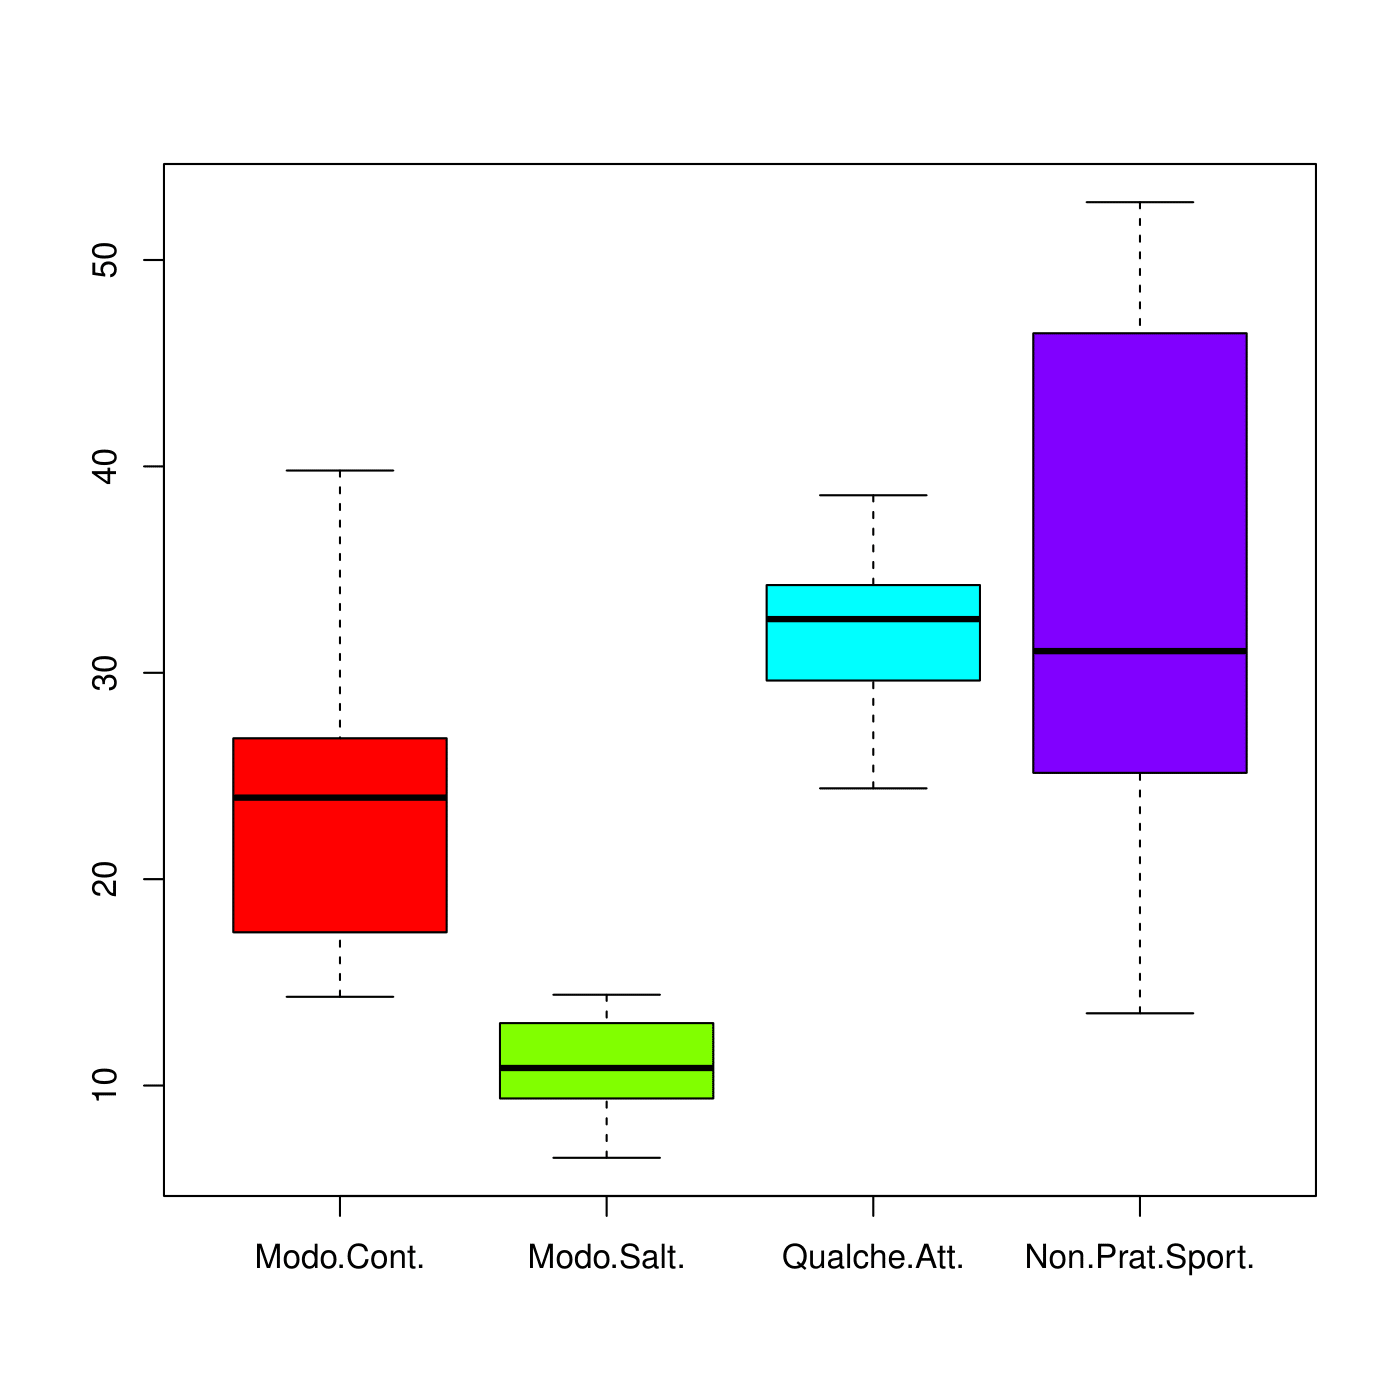
\includegraphics[height=14cm]{ProgettoSAD/capitoli/images/s_desc_univ/quantili_boxplot.png}
    \label{fig:quantili_boxplot}
\end{figure}

Tramite i boxplot ottenuti possiamo fare un'analisi sulla centralità, forma, dispersione e sulla presenza o meno di valori anomali (outlier) della distribuzione di frequenza delle varie caratteristiche. In particolare, si ha che la centralità è espressa dalla mediana. La forma simmetrica o asimmetrica può essere dedotta esaminando le distanze del primo e del terzo quartile dalla linea mediana. I baffi, superiore e inferiore, forniscono informazioni sulla dispersione, sulla forma della distribuzione e anche sulle code della distribuzione. Infatti, la dispersione è deducibile esaminando le distanze del baffo superiore da $Q_3$ e del baffo inferiore da $Q_1$. Inoltre, il baffo inferiore corrisponde al valore più piccolo tra le osservazioni che risulta maggiore o uguale di $Q_1 - 1.5 * (Q_3 - Q_1)$, mentre il baffo superiore corrisponde al valore più grande delle osservazioni che risulta minore o uguale a $Q_3 + 1.5 * (Q_3 - Q_1)$. 

Tra le diverse caratteristiche non sono presenti valori anomali, infatti tutte le caratteristiche rientrano nell'intervallo $Q_1 - 1.5 * (Q_3 - Q_1)$, $Q_3 + 1.5 * (Q_3 - Q_1)$ e i baffi sono posti in corrispondenza del minimo e del massimo.

È presente in tutte le caratteristiche una leggera asimmetria nei dati, poiché la mediana non sembra trovarsi in nessuno dei quattro casi al centro della distribuzione, non essendo dunque utile per avere un valore medio giusto dei dati, ma in tutti i casi il baffo inferiore coincide con il \textit{valore minimo} e il baffo superiore coincide con il \textit{valore massimo}.

Nei casi di svolgimento in Modo Saltuario e Non Praticano Sport la mediana è spostata verso il primo quartile, non risultando utile per avere un valore medio giusto dei dati, mentre nello svolgimento in Modo Continuativo e Qualche Attività la mediana è spostata verso il terzo quartile.

\section{Indici di sintesi: Dispersione dei dati}\label{cap3.2}

Gli indici di posizione non tengono conto della variabilità dei dati; infatti, esistono distribuzioni di frequenza che sono molto diverse tra loro, pur avendo la \textit{stessa media campionaria}. Indici significativi per misurare la variabilità dei dati sono la \textit{varianza campionaria} e la \textit{deviazione standard campionaria}. Tali indici sono detti \textit{indici di dispersione} o \textit{indici di variabilità} poichè misurano la dispersione dei dati \textit{intorno alla media}.

\subsection{Varianza}\label{cap3.2.1}

\noindent \textbf{Definizione:} Assegnato un insieme di dati numerici $x_1, x_2, ..., x_n$, si definisce \textbf{\textit{varianza campionaria}} e si denota con $s^2$ la quantità:

\[s^2 = \frac{1}{n-1} \sum_{i=1}^n (x_i - \bar x)^2 \quad \quad (n = 2, 3, ...) \]

dove $\Bar{x}$ denota la media campionaria dei dati. La varianza identifica il valore della dispersione dei dati intorno al valore medio.

In R la varianza campionaria può essere facilmente calcolata tramite la funzione var().

\vspace{5mm}
\noindent \textbf{Varianza delle caratteristiche del dataset}


\begin{lstlisting}
varianzaCaratteristiche <- function(df) {
  variance <- data.frame(Variance = c(
    var(df$Modo.Cont.),
    +var(df$Modo.Salt.),
    +var(df$Qualche.Att.),
    +var(df$Non.Prat.Sport)))
  row.names(variance) <- names(df)
  variance
}
\end{lstlisting}
\vspace{5mm}

\vspace{5mm}
\begin{tabular}{ c c}
  & Variance\\
 Modo.Cont & 41.671868\\ 
 Modo.Salt & 6.196289\\
 Qualche.Att & 18.043447\\ 
 Non.Prat.Sport & 140.827263\\ 
\end{tabular}
\vspace{5mm}

Dai risultati ottenuti si può notare che la varianza per le frequenze Modo Saltuario e Qualche Attività la varianza è meno elevata, quindi con dati più compatti, mentre per le frequenze Modo Continuativo e Non Praticano Sport la varianza è molto più alta, indicando un maggiore scostamento della media.

\subsection{Deviazione standard}\label{cap3.2.2}

\noindent \textbf{Definizione:} Si definisce \textbf{\textit{deviazione standard campionaria}} e si denota con $s$ la radice quadrata della \textit{varianza campionaria}, ossia:

\[s = \sqrt{\frac{1}{n-1} \sum_{i=1}^n (x_i - \bar x)^2} \quad \quad (n = 2, 3, ...)\]

La deviazione standard è un indice di quanto i numeri si distanzino dalla media aritmetica, cioè quanto i valori di una distribuzione si discostino dalla media stessa. In R la deviazione standard campionaria può essere facilmente calcolata attraverso la funzione \textit{sd()}.

\vspace{5mm}
\noindent \textbf{Deviazione standard delle caratteristiche del dataset}

\vspace{5mm}
\begin{lstlisting}
devStandardCaratteristiche <- function(df) {
  sd <- data.frame(Deviazione_standard = c
  (sd(df$Modo.Cont), sd(df$Modo.Salt.),
   sd(df$Qualche.Att.), sd(df$Non.Prat.Att.)))
  row.names(sd) <- names(df)
  sd
}
\end{lstlisting}
\vspace{5mm}

\vspace{5mm}
\begin{tabular}{ c c}
  & Deviazione Caratteristiche\\
 Modo.Cont & 6.455375\\ 
 Modo.Salt & 2.489235\\
 Qualche.Att & 4.247758\\ 
 Non.Prat.Sport & 11.867066\\ 
\end{tabular}
\vspace{5mm}

\subsection{Coefficiente di variazione}\label{cap3.2.3}

Per confrontare le variazioni esistenti tra diversi campioni di dati è utile introdurre il \textit{coefficiente di variazione}. Esso è un \textit{indice adimensionale} che non dipende dall'unità di misura dei dati. Inoltre, tale indice viene usato anche in insiemi di dati aventi differenti \textit{range di variazione} (il range di variazione è dato dalla differenza tra il massimo e il minimo dei dati.

\noindent \textbf{Definizione:} Assegnato un insieme di dati numerici $x_1, x_2, ..., x_n$, si definisce \textbf{\textit{coefficiente di variazione}} il rapporto tra la \textit{deviazione standard campionaria} e il modulo della \textit{media campionaria}, ossia

\[CV = \frac{s}{|\bar x|}\]

In R non è definita una funzione che calcola il coefficiente di variazione. Tale funzione può essere comunque implementata in R nel seguente modo:

\vspace{5mm}
\begin{lstlisting}
cv <- function(x){
    sd(x)/abs(mean(x))
}
\end{lstlisting}
\vspace{5mm}

\noindent \textbf{Coefficiente di variazione delle caratteristiche del dataset}

\vspace{5mm}
\begin{lstlisting}
coeffVarCaratteristiche <- function(df) {
  cvCoefficient <- data.frame(Variation_Coefficient = c
  (cv(df$Modo.Cont), cv(df$Modo.Salt),
   cv(df$Qualche.Att.), cv(df$Non.Prat.Sport.)))
  row.names(cvCoefficient) <- names(df)
  cvCoefficient
}
\end{lstlisting}
\vspace{5mm}

\vspace{5mm}
\begin{tabular}{ c c}
  & Coefficiente di Variazione\\
 Modo.Cont & 0.2737068\\ 
 Modo.Salt & 0.2274312\\
 Qualche.Att & 0.1334304\\ 
 Non.Prat.Sport & 0.3530814\\ 
\end{tabular}
\vspace{5mm}

Come si evince dai dati ottenuti il coefficiente di variazione più alto si ottiene per la caratteristica Non Praticano Sport, indicando che questi sono i dati che hanno un maggior range di variazione. Inoltre, poichè ogni coefficiente di variazione è inferiore a 1, vuol dire che la media è significativa nei dati.

\section{Forma di una distribuzione di frequenza}\label{cap3.3}

La media e  la mediana sono utili a comprendere la forma delle distribuzioni di frequenza, nel senso che differenze sostanziali tra questi indici indicano uno sbilanciamento eccessivo della distribuzione di frequenza verso destra o verso sinistra. Esistono degli indici statistici che permettono di misurare quando una distribuzione di frequenza presenta simmetria o asimmetria oppure se essa è più o meno piccata.

\subsection{Skewness}\label{cap3.3.1}

La skewness campionaria misura la simmetria di una distribuzione di frequenza.

\noindent \textbf{Definizione:} Assegnato un insieme di dati numerici $x_1, x_2, ..., x_n$, si definisce skewness campionaria il valore:

\[\gamma_1 = \frac{m_3}{m_2^{3/2}}\]

dove $m_3$ denota il momento centrato campionario di ordine 3. In generale, il momento centrato campionario di ordine j è così definito:

\[m_j = 1/n \sum_i=1^n (x_i - \bar x)^j \quad \quad (j = 1, 2, ...)\]

Dalla definizione si ha che:

\begin{itemize}
\item Se $\gamma_1 = 0$ allora la distribuzione di frequenza è simmetrica;
\item Se $\gamma_1 > 0$ allora la distribuzione di frequenza ha la coda di destra più allungata (asimmetria positiva);
\item Se $\gamma_1 < 0$ allora la distribuzione di frequenza ha la coda di sinistra più allungata (asimmetria negativa);
\end{itemize}

In R non esiste una funzione che calcoli la skewness, ma può essere facilmente creata:

\vspace{5mm}
\begin{lstlisting}
skw <- function(x) {
  n <- length(x)
  m2 <- (n - 1) * var(x) / n
  m3 <- (sum((x - mean(x))^3)) / n
  m3 / (m2^1.5)
}
\end{lstlisting}
\vspace{5mm}

Si può ora applicare la funzione alle caratteristiche del dataset, ottenendo:

\vspace{5mm}
\begin{lstlisting}
    skw(df$Modo.Cont.)
    [1] 0.4664549
    skw(df$Modo.Salt.)
    [1] -0.3042624
    skw(df$Qualche.Att.)
    [1] -0.4078287
    skw(df$Non.Prat.Sport.)
    [1] 0.366378
\end{lstlisting}
\vspace{5mm}

Dai risultati ottenuti si ha che le caratteristiche Modo Continuativo e Non Pratica Sport hanno una chiara asimmetria positiva, mentre le caratteristiche Modo Saltuario e Qualche Attività presentano un'asimmetria negativa.

\subsection{Curtosi}\label{cap3.3.2}

La curtosi campionaria permette di misurare la densità dei dati intorno alla media.

\noindent \textbf{Definizione:} Assegnato un insieme di dati numerici $x_1, x_2, ..., x_n$, si definisce curtosi campionaria il valore:

\[\gamma_2 = \beta_2 - 3\]

dove

\[\beta_2 = \frac{m_4}{m_2^2}\]

avendo denotato con $m_4$ il momento centrato campionario di ordine 4. Se risulta:

\begin{itemize}
\item $\beta_2 < 3$, $\gamma_2<0$ allora la distribuzione di frequenza si definisce platicurtica, ossia la distribuzione di frequenza è più piatta di una normale.
\item $\beta_2 > 3$, $\gamma_2 > 0$ allora la distribuzione si definisce leptocurtica, ossia la distribuzione di frequenza è più piccata di una normale;
\item $\beta_2 = 3$, $\gamma_2 = 0$ allora la distribuzione di frequenza si definisce normocurtica, ossia la distribuzione di frequenza è piatta come una normale;
\end{itemize}

Anche in questo caso non esiste una funzione in R che calcoli tale indice, ma può essere così formulata:

\vspace{5mm}
\begin{lstlisting}
curt <- function(x) {
  n <- length(x)
  m2 <- (n - 1) * var(x) / n
  m4 <- (sum((x - mean(x))^4)) / n
  m4 / (m2^2) - 3
}
\end{lstlisting}
\vspace{5mm}

Si può ora applicare la funzione alle caratteristiche del dataset, ottenendo:

\vspace{5mm}
\begin{lstlisting}
    curt(df$Modo.Cont.)
    [1] 0.2121162
    curt(df$Modo.Salt.)
    [1] -1.002682
    curt(df$Qualche.Att.)
    [1] -0.8136908
    curt(df$Non.Prat.Sport.)
    [1] -1.05531
\end{lstlisting}
\vspace{5mm}

La curtosi risulta negativa per le caratteristiche Modo Saltuario, Qualche Attività e Non Pratica Sport, ovvero la distribuzione di frequenza è più piatta di una normale, mentre è positiva per Modo Continuativo, ovvero la distribuzione di frequenza è più piccata di una normale.

\vspace{5mm}
\noindent \textbf{Istogrammi}

Per poter osservare in maniera grafica ciò che si è ottenuto dagli indici di skewness e curtosi campionaria si possono osservare i seguenti istogrammi relativi alle caratteristiche.

\vspace{5mm}
\begin{lstlisting}
istogrammi <- function(df) {
  hist(df$Modo.Cont., freq = TRUE, main = " Istogramma
    Modo Continuativo ", xlab = " Modo Continuativo ", ylab = "
    Percentuale ")
  hist(df$Modo.Salt., freq = TRUE, main = " Istogramma
    Modo Saltuario ", xlab = " Modo Saltuario ", ylab = "
    Percentuale ")
  hist(df$Qualche.Att., freq = TRUE, main = " Istogramma
    Qualche Attivit " , xlab = " Qualche Attività ", ylab = "
    Percentuale ")
  hist(df$Non.Prat.Sport, freq = TRUE, main = " Istogramma
    Non Pratica Sport ", xlab = " Non Pratica Sport ", ylab = "
    Percentuale ")
}
\end{lstlisting}
\vspace{5mm}

Dal codice precedente si ottengono i seguenti istogrammi:

\begin{figure}[!htbp]
    \centering
        \subfloat{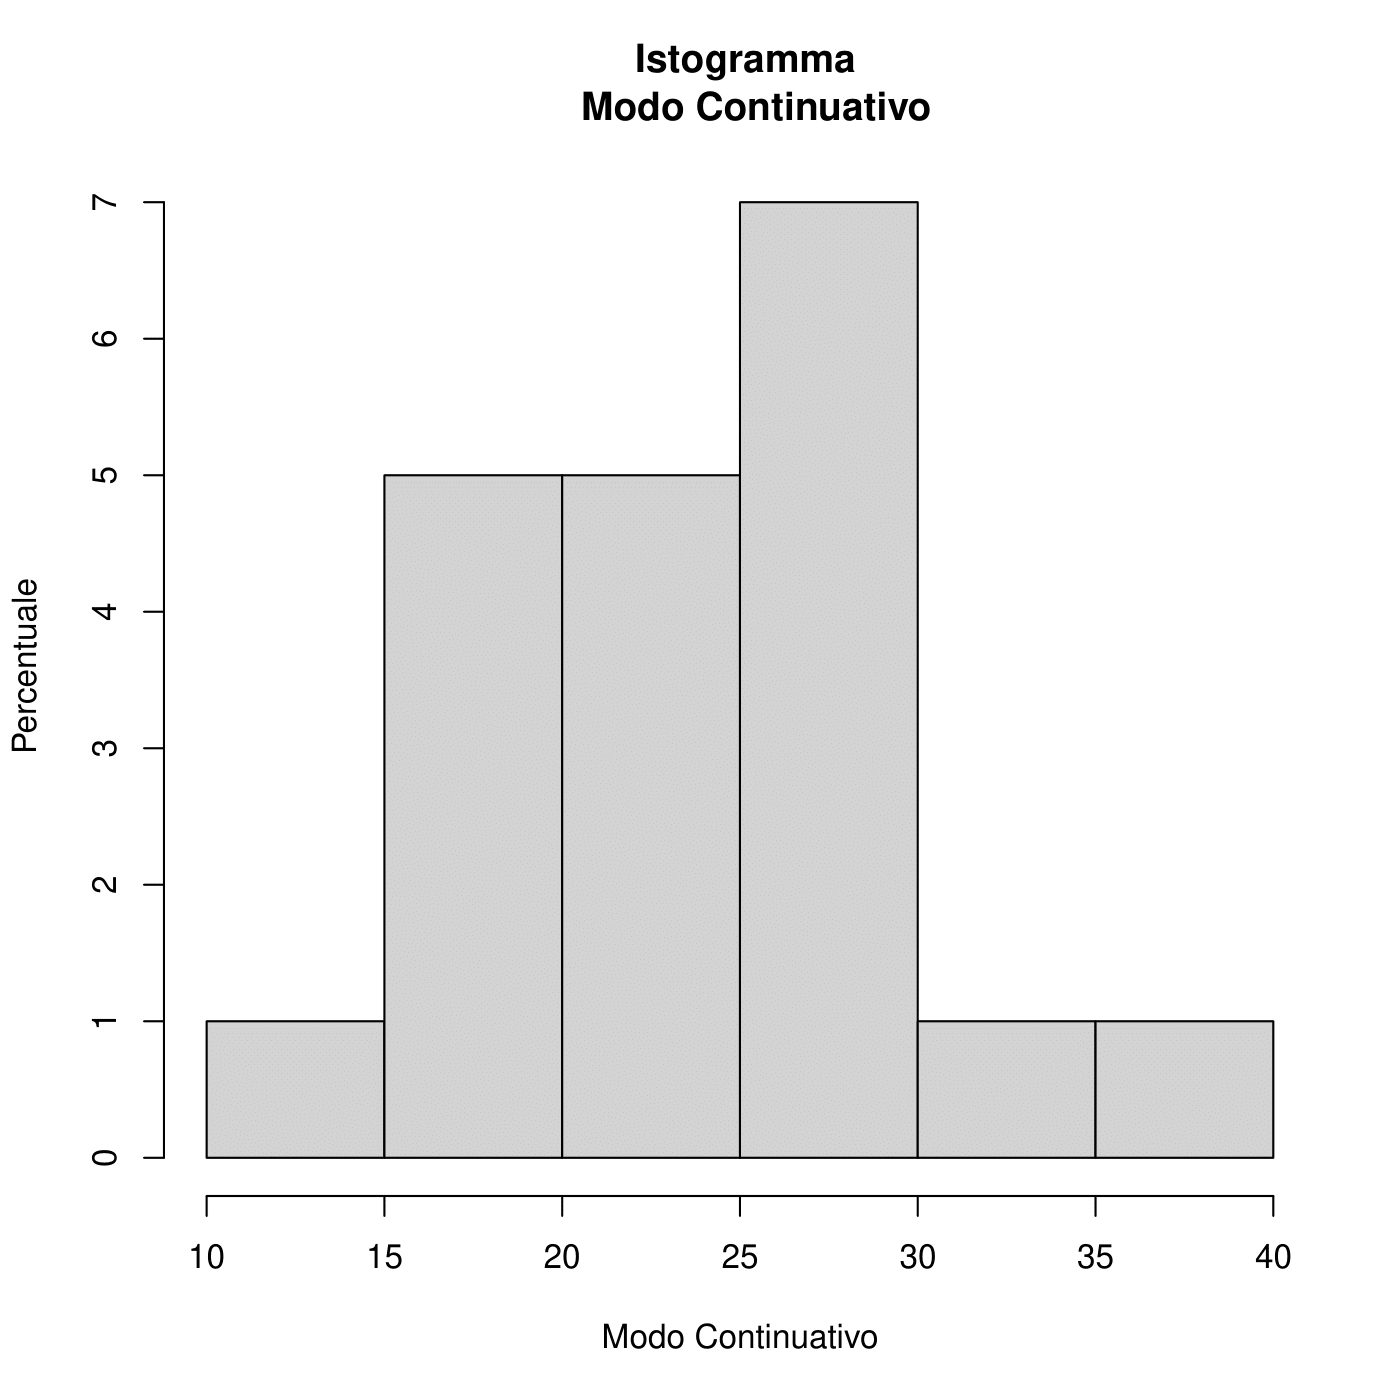
\includegraphics[height=8cm]{ProgettoSAD/capitoli/images/s_desc_univ/hist_modocont.png}}
        \qquad
        \subfloat{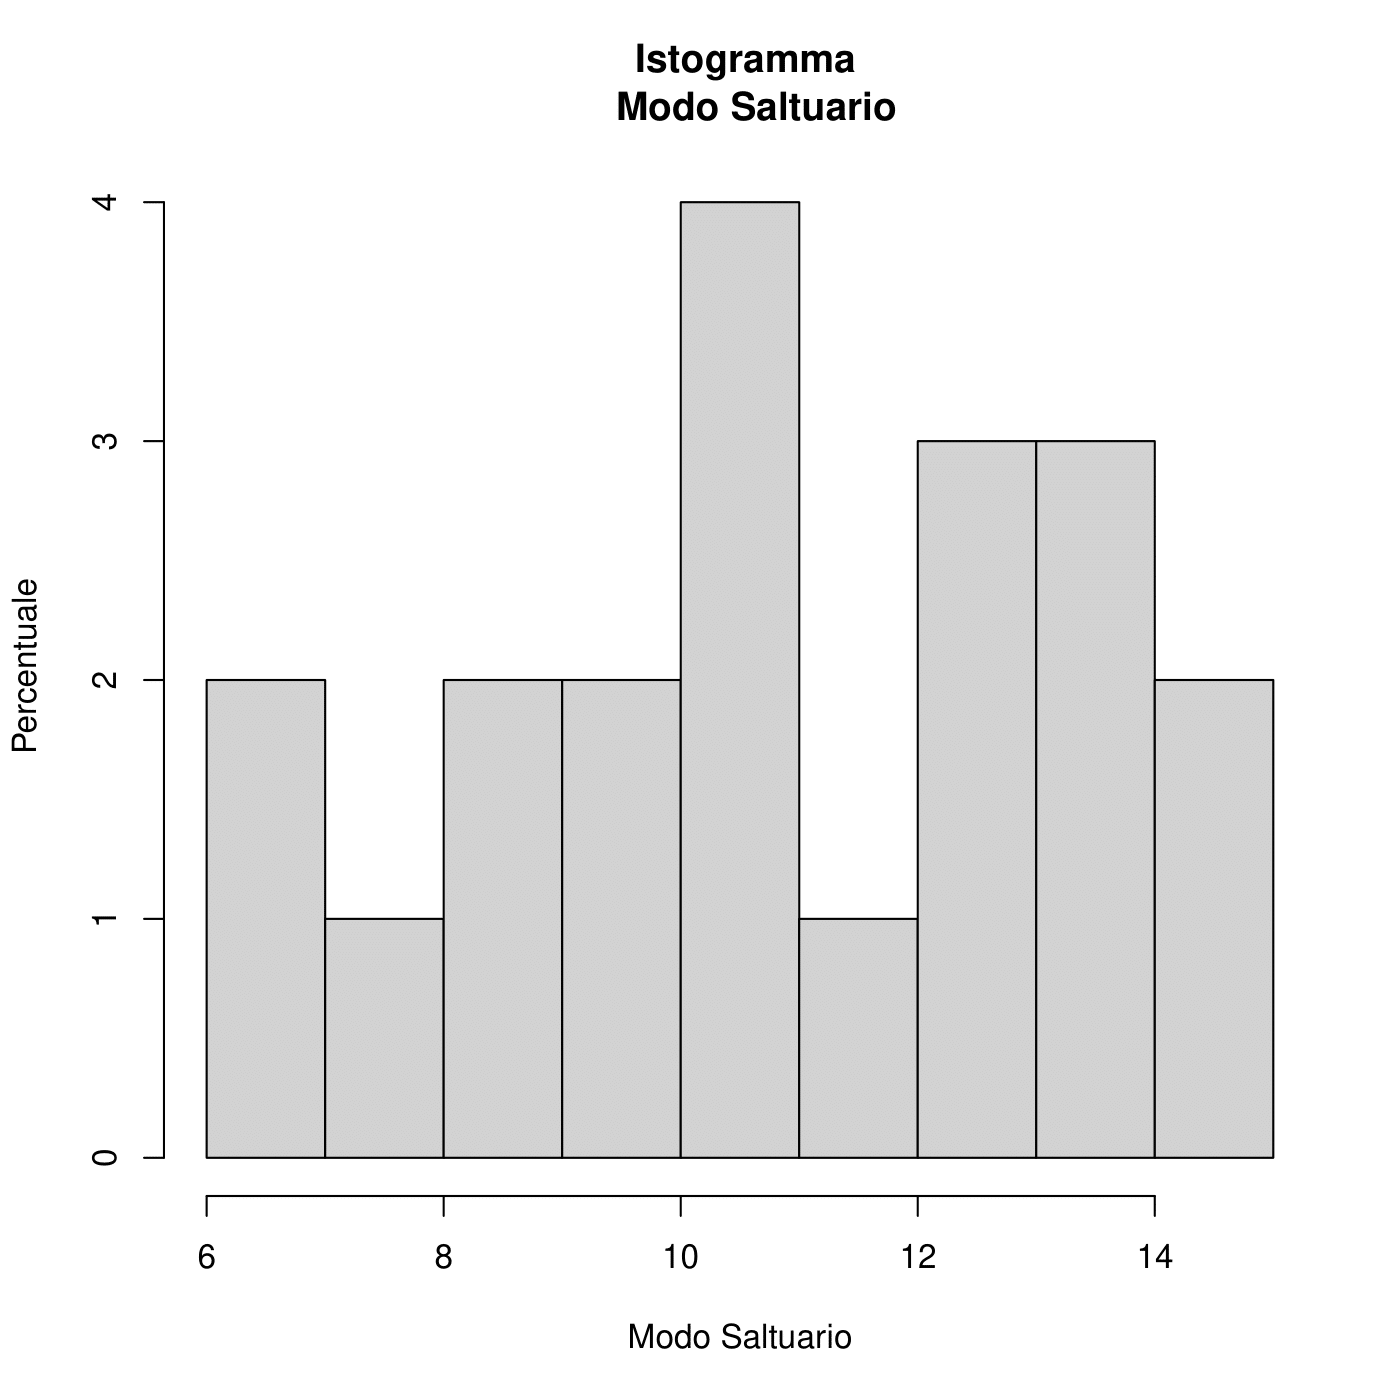
\includegraphics[height=8cm]{ProgettoSAD/capitoli/images/s_desc_univ/hist_modosalt.png}}
        \qquad
\end{figure}
\begin{figure}[!htbp]
    \centering
        \subfloat{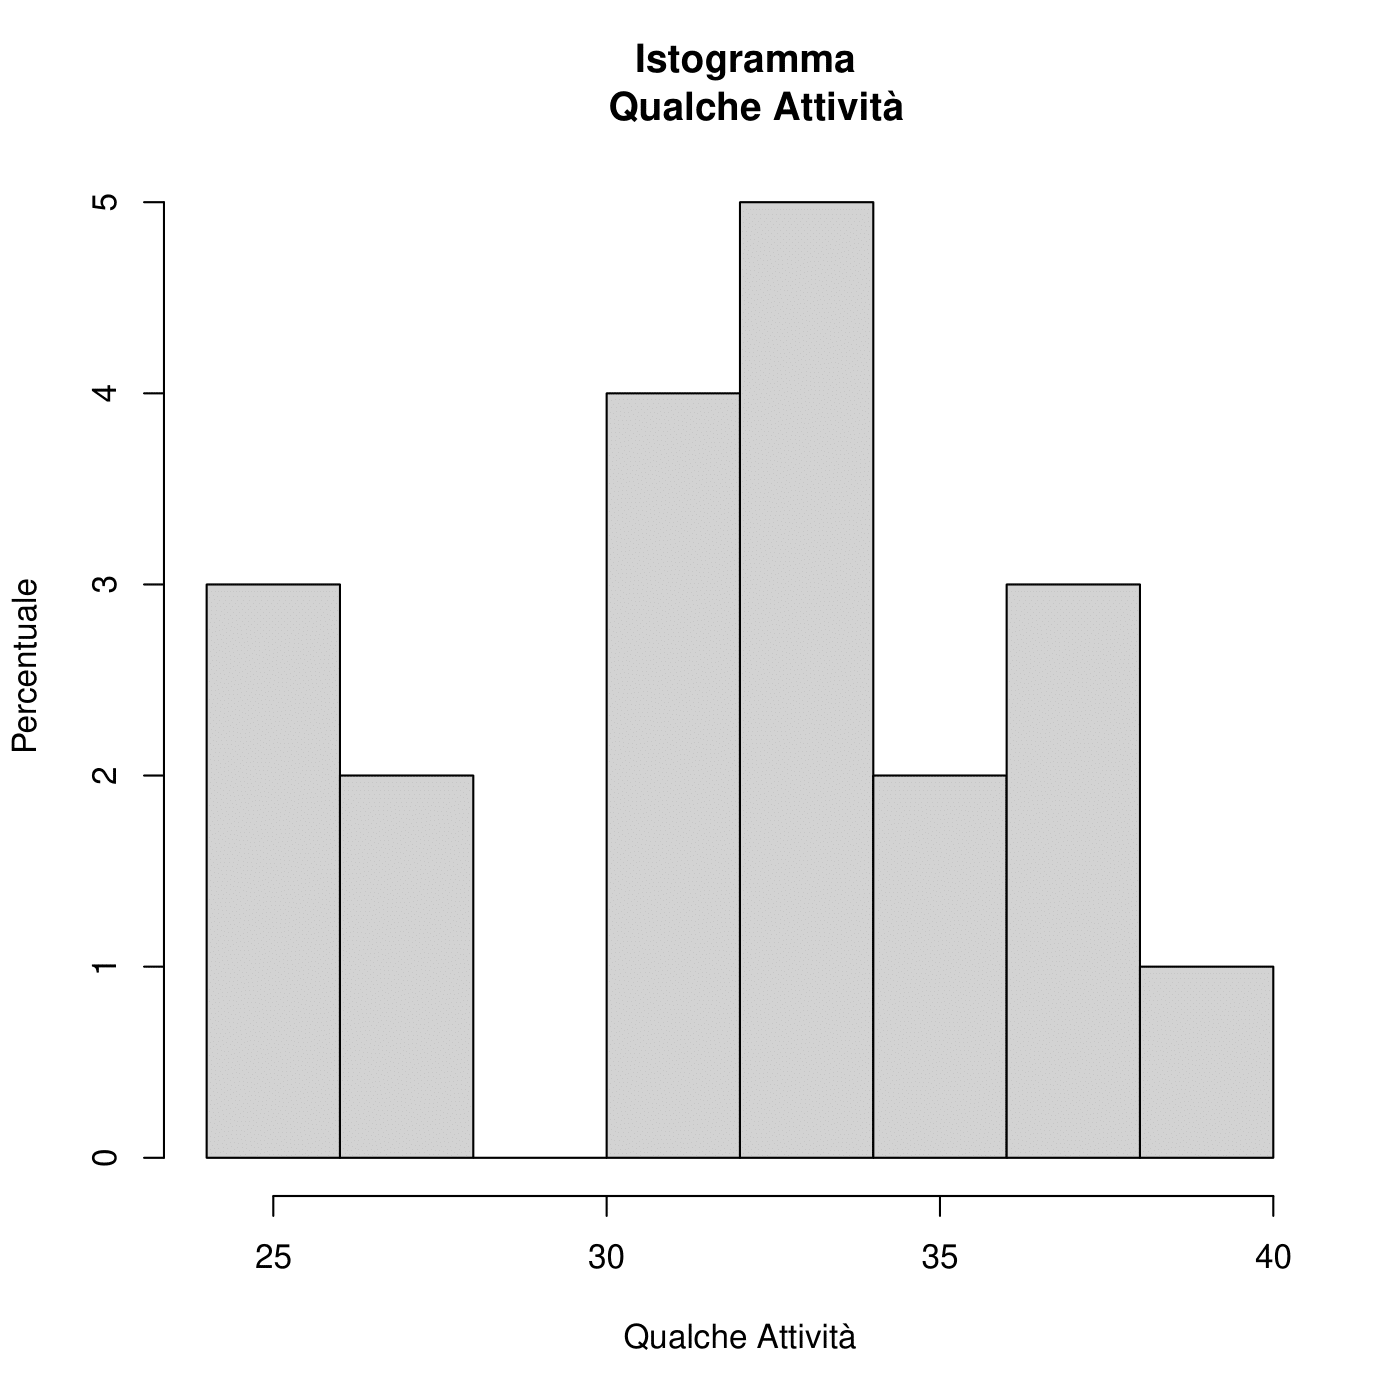
\includegraphics[height=8cm]{ProgettoSAD/capitoli/images/s_desc_univ/hist_qualcheatt.png}}
        \qquad
        \subfloat{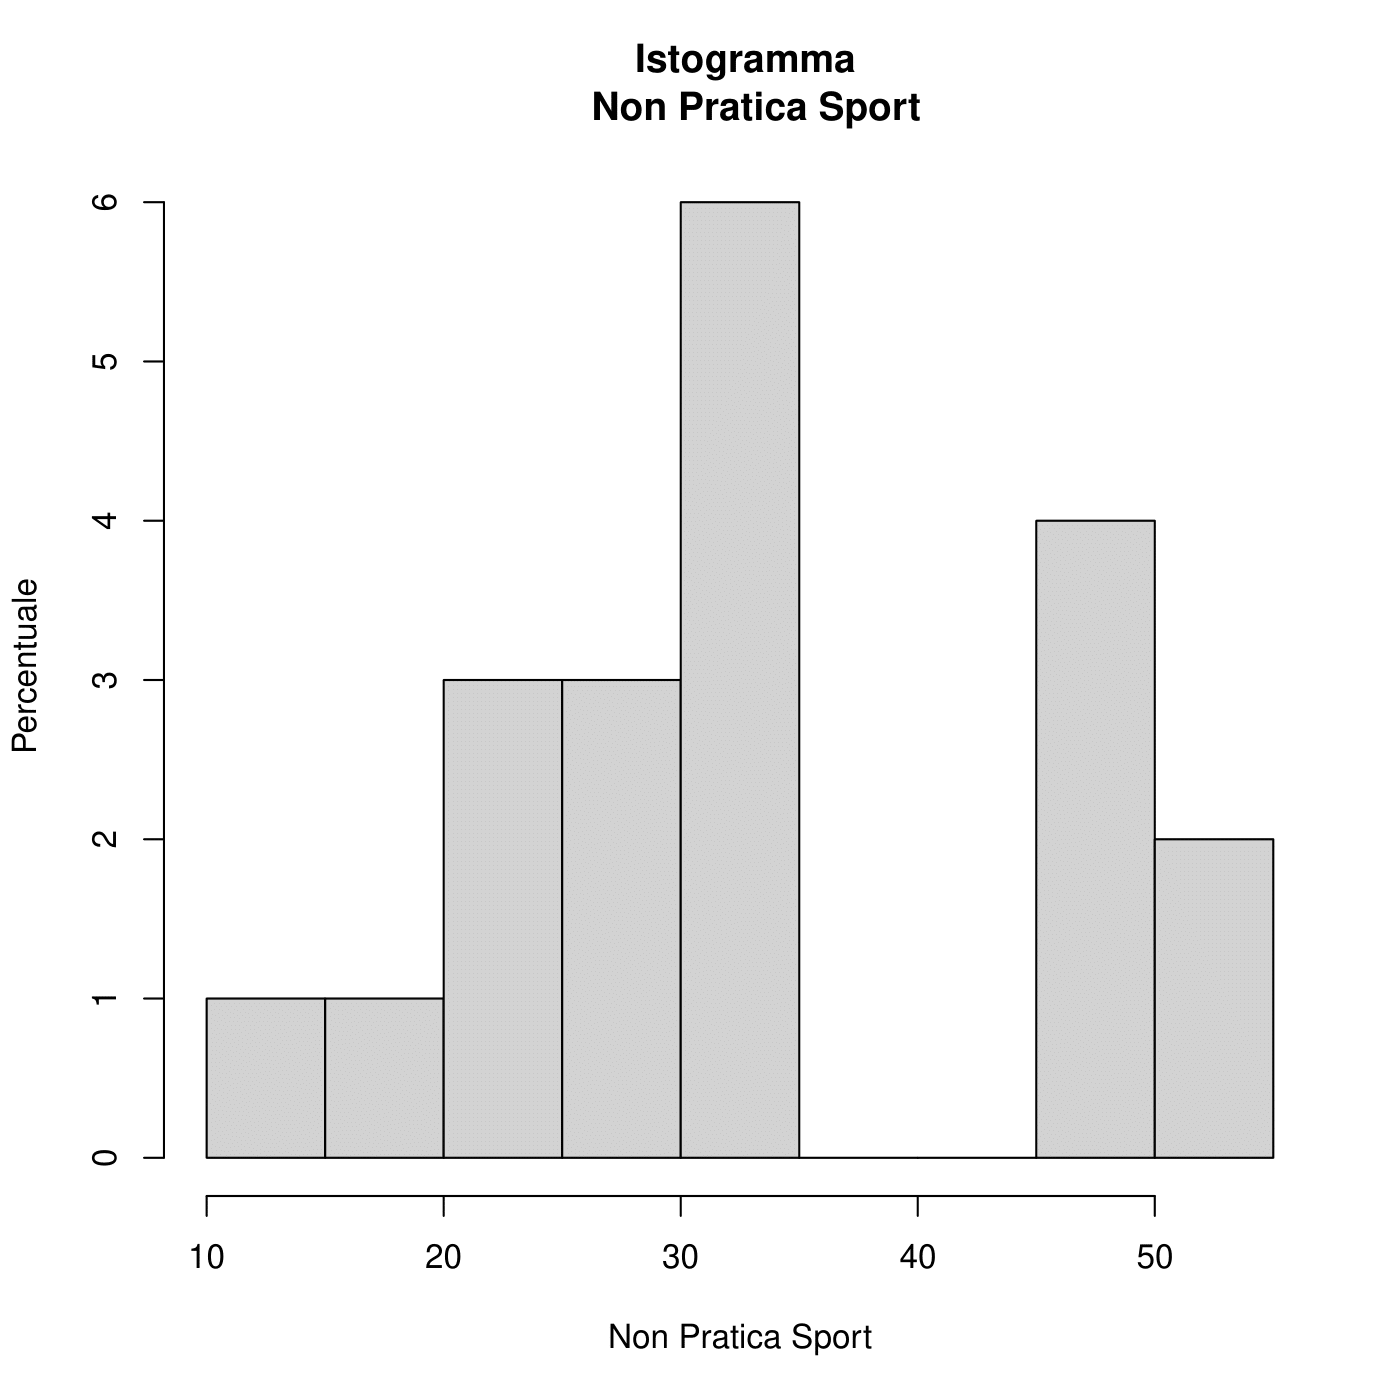
\includegraphics[height=8cm]{ProgettoSAD/capitoli/images/s_desc_univ/hist_nonpratsport.png}}
        \qquad
\end{figure}

%################################################

\newpage